\section{Wprowadzenie}
%\subsection{Machine learning}
%\subsection{Indukcyjne bazy danych}
%\subsection{Zastosowania}

Integracja technologii baz danych z nowoczesnymi metodami
indukcyjnego generowania wiedzy jest naturalnym kierunkiem rozwoju
system�w bazodanowych. Systemy nazywane czasem indukcyjnymi bazami
danych potrafi� odpowiedzie� nie tylko na pytania, dla kt�rych
odpowied� znajduje si� w bazie danych, ale r�wnie� na pytania,
kt�re wymagaj� zsyntetyzowania i zastosowania wiedzy,
wygenerowanej przez indukcyjne wnioskowanie z fakt�w z bazy danych
i wcze�niejszej wiedzy~\cite{bib3}. Schemat typowej indukcyjnej
bazy danych przedstawiony jest na rysunku~\ref{fig:inddb}.

\begin{figure}[!ht]
    \centering
        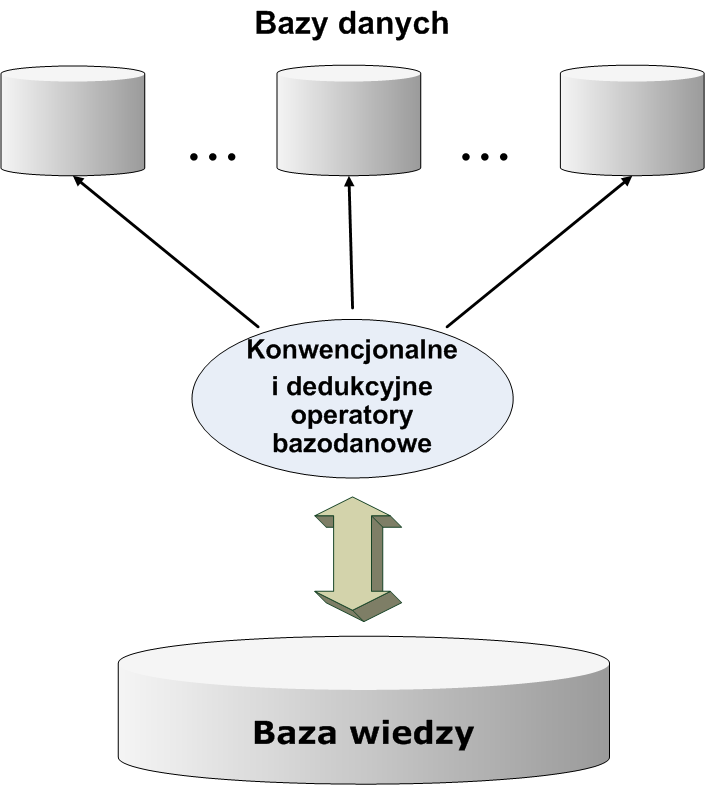
\includegraphics[width=\linewidth]{img/knowledge_mining.png}
    \caption{Indukcyjne bazy danych~\cite{bib2}}
    \label{fig:inddb}
\end{figure}

W niniejszej pracy przedstawiona zosta�a architektura i wybrane
aspekty implementacji platformy \emph{Salomon}, komponentowej
realizacji indukcyjnej bazy danych. Dzi�ki budowie modu�owej uda�o
si� uzyska� du�o lepsz� elastyczno�� systemu w stosunku do innych,
zbli�onych platform.
